\section{Kreativität}
Es gibt in der Literatur nicht DIE Definition von Kreativität. Neben vielen Versuchen von aufstellen allgemeingültiger Definitionen (vgl. Überblcik Krea dfis) und dem forumluieren einer „standard definition of creativity) scheitern viele…

Kreativität soziale Aktivität nach Csik, daher sind Messungen nach dem Grad der kreativität oft abhängig vom jeweiligen Kontext einer jeweiligen Community und schwer zu pauschalisieren.

Die meisten Autoren sind sich jedoch darüber einig, dass kreatitivtät bedeut etwas „neus und innovatives zu schaffen“.
Innerhalb dieser Arbeit fokussieren wir uns auf 3 oft verwendete Frameworks um Kreativität zu beschreiben. Einmal Rhodes 4P. Dieses eigent sich besodners zur strukturellen und vergleichabren Darstellung von Kreativitätsmerkameln.

Guilford 4 phasen kreativer prozess: (a) preparation, (b) incubation, (c) illumination, and (d) verification
Guilford merkamel:
a)	Fluency (many ideas)
b)	Flexibilität (anders denken)
c)	Problemsensitivität (problem erkennen)
d)	Originality
e)	Elaboration
f)	Sensitivity to topic

Torrance macht daraus creativity scored on 4 scales:
Fluency. The total number of interpretable, meaningful, and relevant ideas generated in response to the stimulus.
Flexibility. The number of different categories of relevant responses.
Originality. The statistical rarity of the responses.
Elaboration. The amount of detail in the responses.

Consesnsual assement technicu

Der body of litertur innerhalb der Kreativitä ist enorm. Zudem sind Veröffentlichungen von Diskussionen vom zusammenhang IS/IT und Kreativität in den letzten Jahren stark gesteigen (CSS Shneidernmann). Bei der Vergleichdneden Betrachtung von Kreativitätsexperimenten wird diese vor diesem Hintergrund allerdings aus 3 Blickwinkeln betrachtet, welche hauptsächlich kennzeichnetnd sind: Die Eben der Kreativität, jeweilige Betrachtung welcher 4P und die Operationalisierung bzw. Messung der Kreativität. Veranschaulicht wird dieses im Würfel Abbildung 3. Betrachtet man ein kreatives Produkt kann dieses zb. aus einer Einzelleistung entstehen (Ebene Indivudal), das  Ergbnis 

\begin{mydef}{Kreativität}{def_krea}
  Im Zuge dieser Arbeit impliziert der Begriff „Wirtschaftsinformatik“ die Betrachtung (konstruierter) IT-Artefakte ausschließlich in Form softwareseitiger Anwendungssysteme.
  This theorem is numbered with  \ref{def:def_krea} and is given on page \pageref{def:def_krea}.
\end{mydef}

In der Literatur existeiert trotz vieler Versuche keine einheitliche Definition, wie sich Kreativität definieren lässt. Rhode identifizierte 1961 in diesem Zusammenhang vier Cluster, welche interaktiv auftreten können und aus denen sich das Gesamtkonstrukt der Kreativität bildet. Kreativität kann mdemanch gesehen werden als das Ergebnis kreativer Arbeit und kann selbst kreativ sein. Ein weiterer Forshungsaspket bezieht die kreative Person in den Mittelpunkt, wogegen anderen arbeiten Kreativität als einen Prozess, eine Abfolger kreativer Tätigkeiten sehen,
Diese sogenannten 4P bilden das Grundfundament und diesnen als Basis der Literaturrecherche, indem jedem Paper eine oder mehrer Dimensionen der 4Ps nach Rhode zugeweisenw erden. Alos: Liegt im Fokus des Paper die Person (inwieweit steigert die SW-Lösung die Kreativität einer Person) oder aber das Endresultat (Wie kreativ ist das Endprodukt?). Der kreative Prozess manifestiert sich dabei in erster Linie durch die Wahl der unabhänigen Variablen zb. durch den Einsatz bestimmter Kreativitätstechniken oder Prozessabfolgen.

Kreatives Produkt: Useful, Originality: Entschiedne wird das durch das Fielkd: System Model der Kreativität

Über usefullnes, Effektivität entscheiden die gatekeeper

Die Grundidee des Systemmodells nach Cisk ist jedens, dass neue Ideen um kreativ su sein nicht nu neu sein müssen, sondern auf angebracht und nützlich. Die Effektivität ist demnach durch das soziale Umfeld zu bestimmen, in dem diese neue Ideen ablehnen oder annehmen. Bein Annahme können neue Ideen dann zur bestehenden Wissensbasis (Domäne) hibnzugefügt werden.
\pgfdeclarelayer{edgelayer}
\pgfdeclarelayer{nodelayer}
\pgfsetlayers{edgelayer,nodelayer,main}

\tikzstyle{none}=[inner sep=0pt]
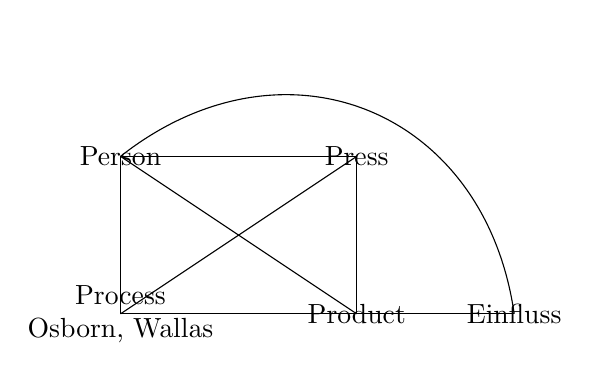
\begin{tikzpicture}
	\begin{pgfonlayer}{nodelayer}
		\node [style=none] (0) at (-8, 3) {Person};
		\node [style=none] (1) at (-5, 3) {Press};
		\node [style=none, align=center] (2) at (-8, 1) {Process \\ Osborn, Wallas};
		\node [style=none] (3) at (-5, 1) {Product};
		\node [style=none] (4) at (-3, 1) {Einfluss};
	\end{pgfonlayer}
	\begin{pgfonlayer}{edgelayer}
		\draw (0.center) to (1.center);
		\draw (0.center) to (2.center);
		\draw (2.center) to (3.center);
		\draw (3.center) to (0.center);
		\draw (2.center) to (1.center);
		\draw (1.center) to (3.center);
		\draw (3.center) to (4.center);
		\draw [bend left=60, looseness=1.25] (0.center) to (4.center);
	\end{pgfonlayer}
\end{tikzpicture}

\begin{tikzcd}
 &  & Person \arrow[dd] \arrow[rr] \arrow[rrdd] &  & Process \arrow[dd] \\
 &  &  &  &  \\
Einfluss \arrow[rr] &  & Produkt \arrow[rr] \arrow[rruu] &  & Press
\end{tikzcd}